\documentclass{beamer}

% \usepackage{beamerthemesplit} // Activate for custom appearance

\title{Remedial Measures, Brown-Forsythe test,F test}
\author{Frank Wood}
%\date{\today}

\newcommand{\comment}[1]{}
\newcommand{\ponedec}{\mathcal{P}^\downarrow_1}
\newcommand{\pone}{\mathcal{P}_1}
\newcommand{\rank}[1]{\mathrm{RANK}\left[#1\right]}
\newcommand{\E}[1]{\mathrm{E}\left[#1\right]}
\newcommand{\py}{\mathcal{PY}}
\newcommand{\iid}{iid.}
\newcommand{\drawiid}{\stackrel{\text{iid}}{\sim}}
\newcommand{\vect}[1]{\mathbf{#1}}
\newcommand{\indicator}[1]{\text{I}\left[ #1 \right]}
\newcommand{\pdcoag}{PD(d_1,0)-\text{COAG}}
\newcommand{\todo}{\textbf{*TODO*}}
\newcommand{\igram}{\text{$\infty$-gram}}
\newcommand{\Prob}{\text{P}}

\def\mm{sequence memoizer }
\def\MM{SM }

\def\pibf{{\boldsymbol{\pi}}}
\def\kapbf{\boldsymbol{\kappa}}
\def\taubf{\boldsymbol{\tau}}
\def\thebf{\boldsymbol{\theta}}
\def\rhobf{\boldsymbol{\rho}}
\def\phibf{\boldsymbol{\phi}}
\def\pbf{\mathbf{p}}
\def\qbf{\mathbf{q}}
\def\sbf{\mathbf{s}}
\def\tbf{\mathbf{t}}
\def\ybf{\mathbf{y}}
\def\wbf{\mathbf{w}}
\def\xbf{\mathbf{x}}
\def\rbf{\mathbf{r}}
\def\tbf{\mathbf{t}}
\def\kbf{\mathbf{k}}
\def\Xbf{\mathbf{X}}
\def\0bf{\mathbf{0}}
\def\Ibf{\mathbf{I}}
\def\phibf{\mathbf{\phi}}
\def\Phibf{\mathbf{\Phi}}
\def\disteq{{\stackrel{D}{=}}}
\def\EE{{\mathbb{E}}}

\def\phiv{\varphi}
\def\phivbf{\boldsymbol{\varphi}}

\def\Ocal{\mathcal{O}}

\DeclareMathOperator*{\Bet}{Beta} \DeclareMathOperator{\coag}{COAG}
\DeclareMathOperator{\frag}{FRAG} \DeclareMathOperator*{\rnk}{RANK}
\DeclareMathOperator*{\gem}{GEM} \DeclareMathOperator*{\pd}{PD}
\DeclareMathOperator*{\gd}{GDir} \DeclareMathOperator*{\Dir}{Dir}
\DeclareMathOperator*{\Ave}{\mathbb{E}}
\DeclareMathOperator*{\Var}{Var}

\begin{document}

\frame{\titlepage}

%\section[Outline]{}
%\frame{\tableofcontents}
%
%\section{Introduction}
%\subsection{Overview of Topics}
%
%\section{Bayesian Analysis}
%\subsection{Single Parameter Model}
\frame[t] {% slide 1
 \frametitle{Remedial Measures}
 \begin{itemize}
  \item How do we know that the regression function is a good
  explainer of the observed data?\\
  - Plotting\\
  - Tests
  \item What if it is not? What can we do about it?\\
  - Transformation of variables(next lecture)
 \end{itemize}
}

\frame[t] {% slide 1
 \frametitle{Graphical Diagnostics for the Predictor Variable}
 \begin{itemize}
  \item Dot Plot\\
  - Useful for visualizing distribution of inputs
  \item Sequence Plot\\
  - Useful for visualizing dependencies between error terms
  \item Box Plot
  - Useful for visualizing distribution of inputs
 \end{itemize}
 Toluca manufacturing example again: production time vs. lot size
}

\frame[t] {% slide 1
 \frametitle{Dot Plot}
 \begin{figure}[h!]
   \centering
     \caption{}
     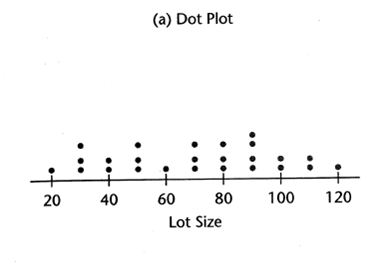
\includegraphics[scale=.4]{4.png}
 \end{figure}
 \begin{itemize}
 \item How many observations per input value?
 \item Range of inputs?
 \end{itemize}
}

\frame[t] {
 \frametitle{Sequence Plot}
 \begin{figure}[h!]
   \centering
     \caption{}
     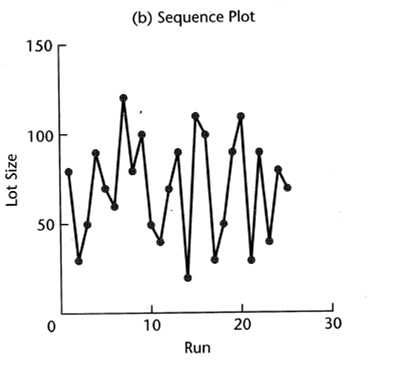
\includegraphics[scale=.4]{5.png}
 \end{figure}
 \begin{itemize}
 \item If observations are made over time, is there a correlation
 between input and position in observation sequence?
 \end{itemize}
}

\frame[t] {
 \frametitle{Box Plot}
  \begin{figure}[h!]
   \centering
     \caption{}
     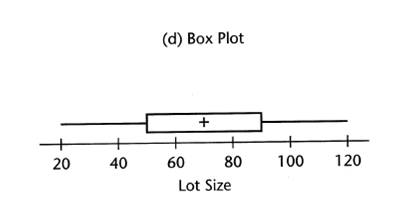
\includegraphics[scale=.4]{6.png}
 \end{figure}
 \begin{itemize}
 \item Shows\\
 - Median\\
 - 1st and 3rd quartiles\\
 - Maximum and minimum
 \end{itemize}
}

\frame[t] {
 \frametitle{Residuals}
 \begin{itemize}
 \item Remember, the definition of residuals:\\
 \begin{center}
 $e_i=Y_i-\hat{Y_i}$
 \end{center}
 \item And the difference between that and the unknown true error\\
 \begin{center}
 $\epsilon=Y_i-E(Y_i)$
 \end{center}
 \item In a normal regression model the $\epsilon_i$'s are assumed
 to be iid $N(0,\sigma^2)$ random variables. The observed residuals
 $e_i$ should reflect these properties.
 \end{itemize}
}

\frame[t] {
 \frametitle{Remember: residual properties}
 \begin{itemize}
 \item Mean\\
 \begin{center}
 $\bar{e_i}=\frac{\sum e_i}{n}=0$
 \end{center}
 \item Variance\\
 \begin{center}
 $s^2=\frac{(e_i-\bar{e})^2}{n-2}=\frac{SSE}{n-2}=MSE$
 \end{center}
 \end{itemize}
}

\frame[t] {
 \frametitle{Nonindependence of Residuals}
 \begin{itemize}
 \item The residuals $e_i$ are not independent random variables
 - The fitted values $\hat{Y_i}$ are based on the same fitted
 regression line.\\
   - The residuals are subject to two constraints \\
 \begin{enumerate}
\item     - Sum of the $e_i$'s equals 0
 \item    - Sum of the products $X_i e_i$'s equals 0
\end{enumerate}

 \item When the sample size is large in comparison to the number of
 parameters in the regression model, the dependency effect among the
 residuals $e_i$ can reasonably safely be ignored.
 \end{itemize}
}

\frame[t] {
 \frametitle{Definition: semistudentized residuals}
 \begin{itemize}
 \item It may be useful sometimes to look at a standardized set of residuals, for instance in outlier detection.
 \item Like usual, since the standard deviation of $\epsilon_i$ is
 $\sigma$(itself estimated by square root of MSE) a natural form of
 standardization to consider is
 \begin{center}
 $e_i^{\ast}=\frac{e_i}{\sqrt{MSE}}$
 \end{center}
 \item This is called a semistudentized residual.
 \end{itemize}
}

\frame[t] {
 \frametitle{Departures from Model...}
 To be studied by residuals
 \begin{itemize}
 \item Regression function not linear
 \item Error terms do not have constant variance
 \item Error terms are not independent
 \item Model fits all but one or a few outlier observations
 \item Error terms are not normally distributed
 \item One or more predictor variables have been omitted from the
 model
 \end{itemize}
}

\frame[t] {
 \frametitle{Diagnostics for Residuals}
 \begin{itemize}
 \item Plot of residuals against predictor variable
 \item Plot of absolute or squared residuals against predictor
 variable
 \item Plot of residuals against fitted values
 \item Plot of residuals against time or other sequence
 \item Plot of residuals against omitted predictor variables
 \item Box plot of residuals
 \item Normal probability plot of residuals
 \end{itemize}
}

\frame[t] {
 \frametitle{Diagnostic Residual Plots}
  \begin{figure}[h!]
   \centering
     \caption{Toluca example: labor time vs. lot size}
     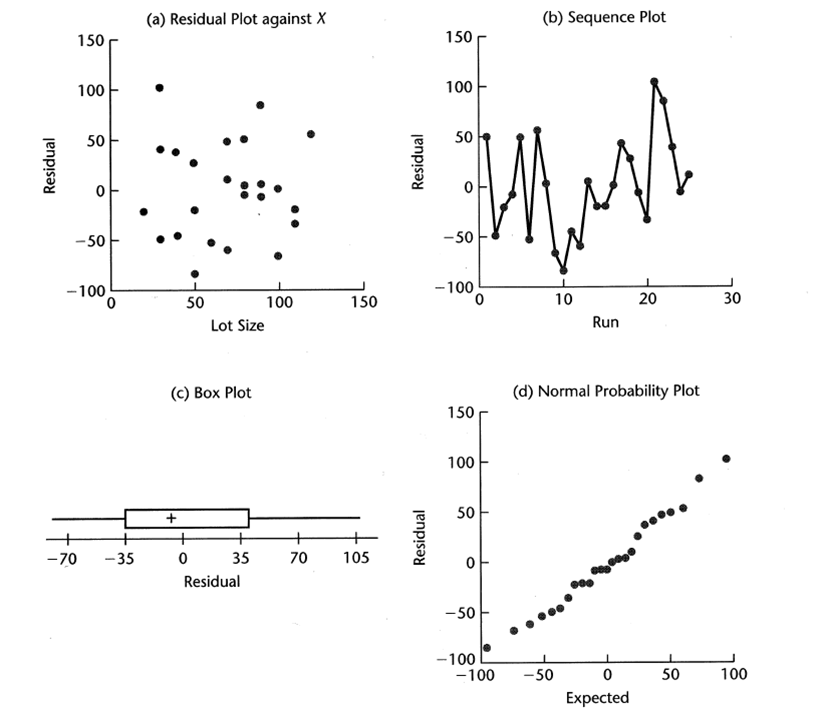
\includegraphics[scale=.4]{13.png}
 \end{figure}
}

\frame[t] {
 \frametitle{Scatter and Residual Plot}
  \begin{figure}[h!]
   \centering
     \caption{Transit example : ridership increase vs. num. maps distributed}
     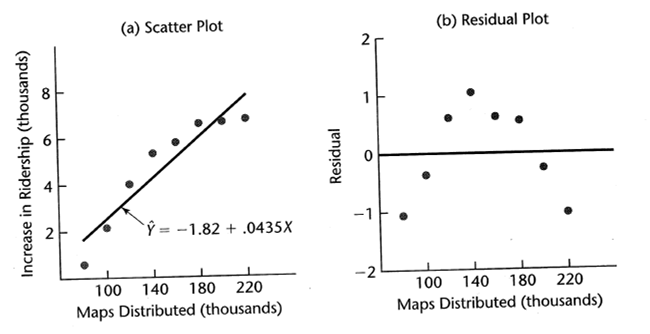
\includegraphics[scale=.4]{14.png}
 \end{figure}
}

\frame[t] {
 \frametitle{Prototype Residual Plots}
  \begin{figure}[h!]
   \centering
     \caption{Indicate residual plots}
     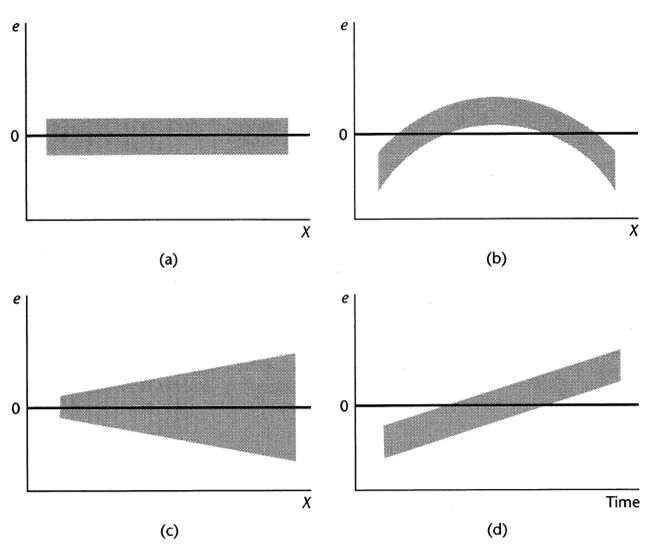
\includegraphics[scale=.4]{15.png}
 \end{figure}
}

\frame[t] {
 \frametitle{Nonconstancy of Error Variance}
  \begin{figure}[h!]
   \centering
    % \caption{}
     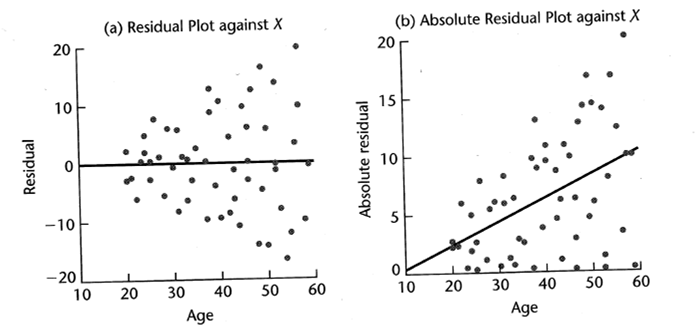
\includegraphics[scale=.4]{16.png}
 \end{figure}
}

\frame[t] {
 \frametitle{Presence of Outliers}
 \begin{figure}[h!]
   \centering
  %   \caption{}
     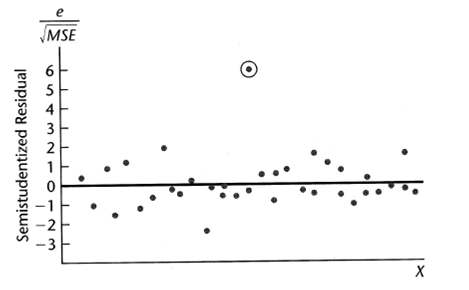
\includegraphics[scale=.4]{17.png}
 \end{figure}
 Outliers can strongly effect the fitted values of the regression
 line.
}

\frame[t] {
 \frametitle{Outlier effect on residuals}
 \begin{figure}[h!]
   \centering
   %  \caption{}
     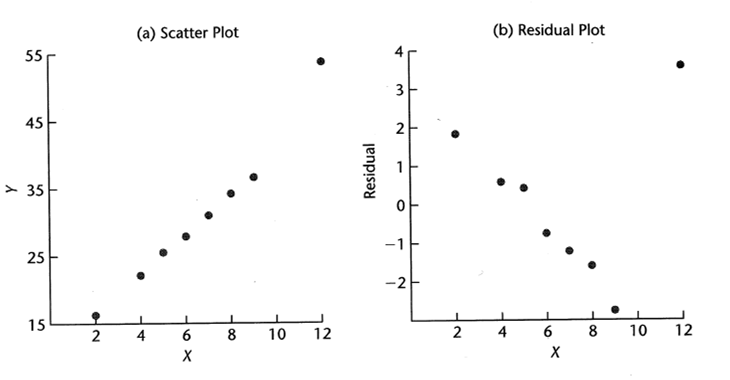
\includegraphics[scale=.4]{18.png}
 \end{figure}
}

\frame[t] {
 \frametitle{Nonindependence of Error Terms}
  \begin{figure}[h!]
   \centering
   %  \caption{}
     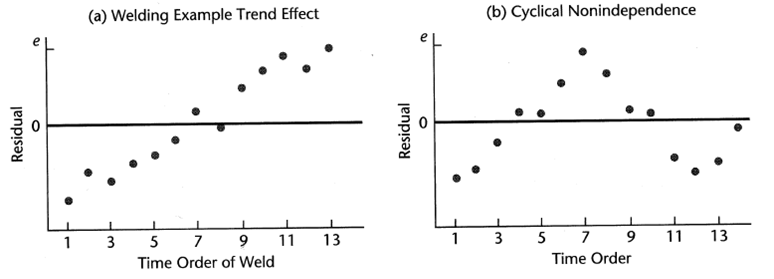
\includegraphics[scale=.4]{19.png}
 \end{figure}
 Sequential observations can exhibit observable trends in error distribution.
}

\frame[t] {
 \frametitle{Non-normality of Error Terms}
 \begin{itemize}
 \item Distribution plots
 \item Comparison of Frequencies
 \item Normal probability plot \\
 -Q-Q plot with numerical quantiles on the horizontal axis
 \end{itemize}
  \begin{figure}[h!]
   \centering
     \caption{Examples of non-normality in distribution of error terms}
     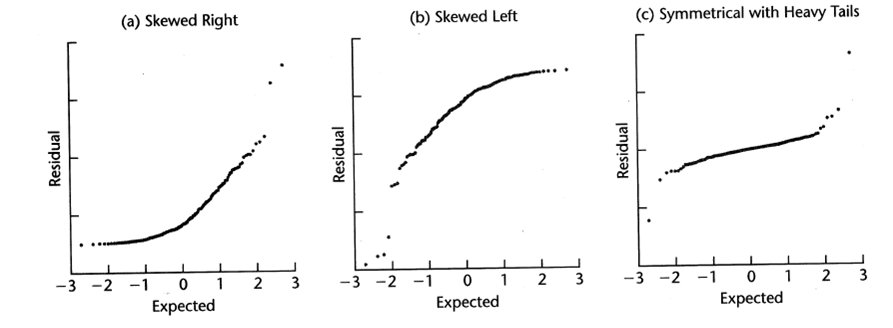
\includegraphics[scale=.4]{20.png}
 \end{figure}
}

\frame[t] {
 \frametitle{Normal probability plot}
 \begin{itemize}
 \item For a $N(0,MSE^{1/2})$ random variable, a good approximation
 of the expected value of the k-th smallest observation in a random
 sample of size n is
 \begin{center}
 $\sqrt{MSE}[z(\frac{k-.375}{n+.25})]$
 \end{center}
 \item A normal probability plot consists of plotting the expected
 value of the k-th smallest observation against the observed k-th
 smallest observation
 \end{itemize}
}

\frame[t] {
 \frametitle{Omission of Important Predictor Variables}
 \begin{columns}
\begin{column}{.5\linewidth}
\begin{itemize}
\item Example\\
- Qualitative variable\\
  - Type of machine
\item Partitioning data can reveal dependence on omitted variable(s)
\item Works for quantitative variables as well
\item Can suggest that inclusion of other inputs is important
\end{itemize}
\end{column}
\begin{column}{.5\linewidth}
  \begin{figure}[h!]
   \centering
     \caption{}
     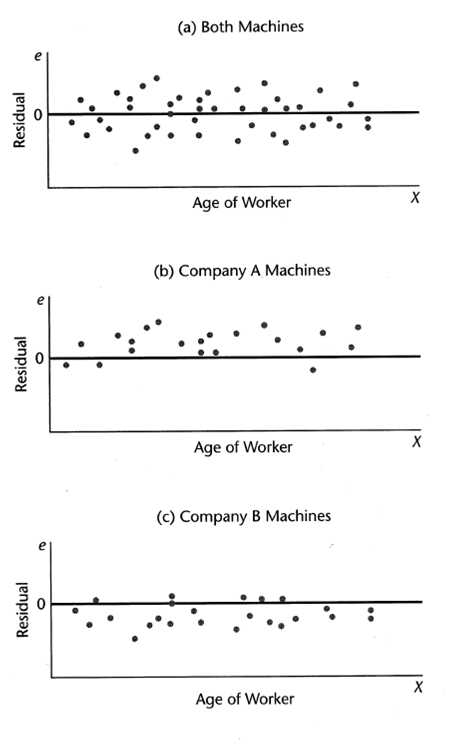
\includegraphics[scale=.4]{22.png}
 \end{figure}
\end{column}
\end{columns}
}

\frame[t] {
 \frametitle{Tests Involving Residuals}
 \begin{itemize}
 \item Tests for randomness
 \item Tests for constancy of variance
 \item Tests for outliers
 \item Tests for normality of error distribution
 \end{itemize}
}

\frame[t] {
 \frametitle{Correlation Test for Normality of Error Distribution}
 \begin{columns}
\begin{column}{.5\linewidth}
\begin{itemize}
\item A formal test for the normality of the error terms can be developed in terms of the 
correlation between the ordered observed errors 

\item Tables(B.6 in the book) given critical values for the null
hypothesis (normally distributed errors) holding.
\end{itemize}
\end{column}
\begin{column}{.5\linewidth}
  \begin{figure}[t!]
   \centering
     \caption{}
     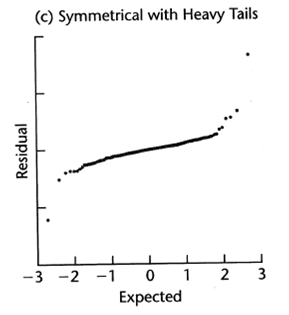
\includegraphics[scale=.4]{24.png}
 \end{figure}
\end{column}
\end{columns}
}

\frame[t] {
 \frametitle{Correlation Test for Normality of Error Distribution}

For one way to run this correlation test let 

\[\{e_{\sigma(1)}, \ldots, e_{\sigma(n)}\} \] be the permutation of the observed errors such that $e_{\sigma(j)} \leq e_{\sigma(j)} \forall j$ and $\sigma:\mathbb{Z}\rightarrow\mathbb{Z}$ is a permutation. Let
\[\{r_1, \ldots, r_k, \ldots, r_n\} \] be the expected value of the $k^{th}$ residual under the normality assumption, i.e.
\[ r_k \approx \sqrt{MSE}[z(\frac{k-.375}{n+.25})]\]
Then compute the (sample) correlation between these sets of random variables.  The sample correlation can be found by replacing the covariance and variance functions with their sample estimates in 
\[ \rho(Y,Z) = \frac{\sigma\{Y,Z\}}{\sigma\{Y\}\sigma\{Z\}}\]

}

\frame[t] {
 \frametitle{Tests for Constancy of Error Variance}
 \begin{itemize}
 \item Brown-Forsythe test does not depend normality of error terms. The Brown-Forsythe test is applicable to simple linear
   regression when\\
  \begin{itemize}
\item     The variance of the error terms either increases or
     decreases with X (``megaphone'' residual plot)\\
 \item    Sample size is large enough to ignore dependencies between
     the residuals
\end{itemize}

 \item The Brown-Forsythe test is essentially a t-test for testing whether the means of two
 normally distributed populations are the same where the populations are the absolute deviations between the prediction and the observed output space in two non-overlapping partitions of the input space.
 \end{itemize}
}

\frame[t] {
 \frametitle{Brown-Forsythe Test}
 \begin{itemize}
 \item Divide X into $X_1$ (the low values of X) and $X_2$ (the high values of X)
 \item Let $e_{i1}$ be the error terms for $X_1$ and vice versa
 \item let $n=n_1+n_2$
 \item The Brown-Forsythe test uses the absolute deviations of the
 residuals around their group median
 \begin{center}
 $d_{1i}=|e_{1i}-\tilde{e_1}|$
 \end{center}
 \end{itemize}
}

\frame[t] {
 \frametitle{Brown-Forsythe Test}
 \begin{itemize}
 \item The test statistic for comparing the means of the absolute
 deviations of the residuals around the group medians is
 \begin{center}
 $t_{BF}^{\ast}=\frac{\bar{d_1}-\bar{d_2}}{s\sqrt{\frac{1}{n_1}+\frac{1}{n_2}}}$
 \end{center}
 where
 \begin{center}
 $s^2=\frac{\sum(d_{i1}-\bar{d_1})^2+\sum(d_{i1}-\bar{d_1})^2}{n-2}$
 \end{center}
 \end{itemize}
}

\frame[t] {
 \frametitle{Brown-Forsythe Test}
 \begin{itemize}
 \item If $n_1$ and $n_2$ are not extremely small
 \begin{center}
 $t_{BF}^{\ast}~\sim~t(n-2)$
 \end{center}
 approximately
 \item From this confidence intervals and tests can be constructed.
 \end{itemize}
}

\frame[t] {
 \frametitle{F test for lack of fit}
 \begin{itemize}
 \item Formal test for determining whether a specific type of
 regression function adequately fits the data.
 \item Assumptions (usual):\\
 - observations $Y|X$ are 
  \begin{enumerate}
\item   i.i.d.
 \item   normally distributed
  \item  same variance $\sigma^2$
\end{enumerate}

 \item Requires: repeat observations at one or more X levels (called replicates)
 \end{itemize}
}

\frame[t] {
 \frametitle{Example}
 \begin{itemize}
 \item 12 similar branches of a bank offered gifts for setting up
 money market accounts
 \item Minimum initial deposits were specific to qualify for the
 gift
 \item Value of gift was proportional to the specified minimum
 deposit
 \item Interested in: relationship between specified minimum
 deposit and number of new accounts opened
 \end{itemize}
}

\frame[t] {
 \frametitle{F Test Example Data and ANOVA Table}
\begin{figure}[h!]
   \centering
     \caption{}
     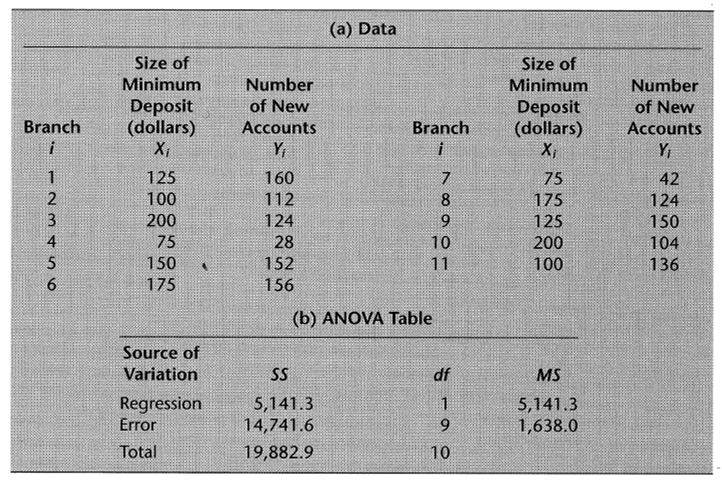
\includegraphics[scale=.4]{31.png}
 \end{figure}
}

\frame[t] {
 \frametitle{Fit}
\begin{figure}[h!]
   \centering
     \caption{}
     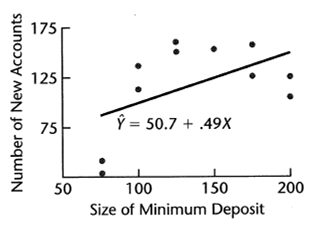
\includegraphics[scale=.4]{32.png}
 \end{figure}
}

\frame[t] {
 \frametitle{Data Arranged To Highlight Replicates}
\begin{figure}[h!]
   \centering
     \caption{}
     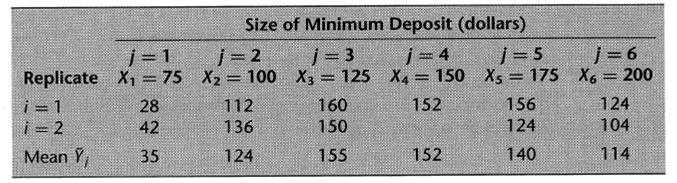
\includegraphics[scale=.4]{33.png}
 \end{figure}
 \begin{itemize}
 \item The observed value of the response variable for the i-th
 replicate for the j-th level of X is $Y_{ij}$
 \item The mean of the Y observations at the level $X=X_j$ is $\bar{Y_j}$
 \end{itemize}
}

\frame[t] {
 \frametitle{Full Model vs. Regression Model}
 \begin{itemize}
 \item The full model is
 \begin{center}
 $Y_{ij}=\mu_j+\epsilon_{ij}$~~~~~~~~~~Full model
 \end{center}
 where\\
 - $\mu_j$ are parameters $j=1,...,c$\\
 - $\epsilon_{ij}$ are iid $N(0,\sigma^2)$
 \item Since the error terms have expectation zero
 \begin{center}
 $E(Y_{ij})=\mu_{j}$
 \end{center}
 \end{itemize}
}

\frame[t] {
 \frametitle{Full Model}
 \begin{itemize}
 \item In the full model there is a different mean (a free parameter)
 for each $X_i$
 \item In the regression model the mean responses are constrained to
 lie on a line
 \begin{center}
 $E(Y)=\beta_0+\beta_1 X$
 \end{center}
 \end{itemize}
}

\frame[t] {
 \frametitle{Fitting the Full Model}
 \begin{itemize}
 \item The estimators of $\mu_j$ are simply
 \begin{center}
 $\hat{\mu_j}=\bar{Y_j}$
 \end{center}
 \item The error sum of squares of the full model therefore is
 \begin{center}
 $SSE(F)=\sum\sum(Y_{ij}-\bar{Y_j})^2==SSPE$
 \end{center}
 \end{itemize}
}

\frame[t] {
 \frametitle{Degrees of Freedom}
 \begin{itemize}
 \item Ordinary total sum of squares had n-1 degrees of freedom.
 \item Each of the j terms is a ordinary total sum of squares\\
 - Each then has $n_j-1$ degrees of freedom
 \item The number of degrees of freedom of SSPE is the sum of the
 component degrees of freedom
 \begin{center}
 $df_F=\displaystyle\sum_j (n_j-1)=\displaystyle\sum_j n_j -c=n-c$
 \end{center}
 \end{itemize}
}

\frame[t] {
 \frametitle{General Linear Test}
 \begin{itemize}
 \item Remember: the general linear test proposes a reduced model
 null hypotheses\\
 - this will be our normal regression model
 \item The full model will be as described (one independent mean for each level of X)
 \begin{center}
 $H_0: E(Y)=\beta_0+\beta_1 X$\\
 $H_a: E(Y)\not= \beta_0+\beta_1 X$
 \end{center}
 \end{itemize}
}

\frame[t] {
 \frametitle{SSE For Reduced Model}
 The SSE for the reduced model is as before\\
 - remember
 \begin{center}
 \begin{align*}
 SSE(R)&=\sum_i\sum_j[Y_{ij}-(b_0+b_1 X_j)]^2\\
       &=\sum_i\sum_j(Y_{ij}-\hat{Y_{ij}})^2
 \end{align*}
 \end{center}
 - and has n-2 degrees of freedom $df_R=n-2$
}

\frame[t] {
 \frametitle{SSE(R)}
 \begin{figure}[h!]
   \centering
     \caption{}
     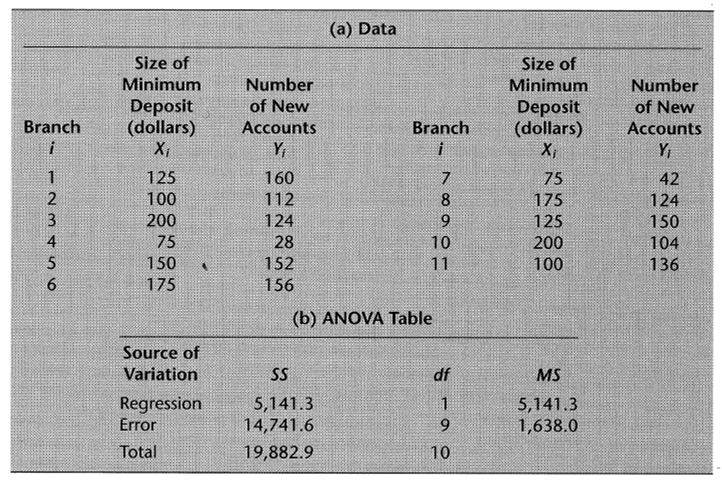
\includegraphics[scale=.4]{40.png}
 \end{figure}
}

\frame[t] {
 \frametitle{F Test Statistic}
 From the general linear test approach
 \begin{center}
 $F^\ast=\frac{SSE(R)-SSE(F)}{df_R-df_F}\div\frac{SSE(F)}{df_F}$\\
 $F^\ast=\frac{SSE-SSPE}{(n-2)-(n-c)}\div\frac{SSPE}{n-c}$
 \end{center}
 where a little algebra takes us to the next slide
}

\frame[t] {
 \frametitle{F Test Rule}
 \begin{itemize}
 \item From the F test we know that large values of $F^\ast$ lead us
 to reject the null hypothesis:\\
 If $F^\ast \le F(1-\alpha;c-2,n-c)$, conclude $H_0$\\
 If $F^\ast > F(1-\alpha;c-2,n-c)$, conclude $H_a$
 \item For this example we have
\begin{figure}[h!]
   \centering
     
     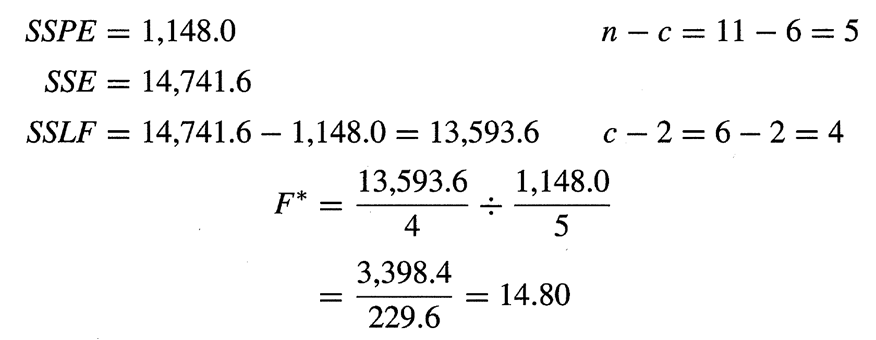
\includegraphics[scale=.4]{42.png}
 \end{figure}
 \end{itemize}
}

\frame[t] {
 \frametitle{Example Conclusion}
 \begin{itemize}
 \item If we set the significance level to $\alpha=.01$
 \item And look up the value of the F inv-cdf $F(.99,4,5)=11.4$
 \item We can conclude that the null hypothesis should be rejected.
 \end{itemize}
}








\end{document}
